%%%%%%%%%%%%%%%%%%%%%%%%%%%%%%%%%%%%%%%%%%%%%%%%%%%%%%%%%%%%%
%% HEADER
%%%%%%%%%%%%%%%%%%%%%%%%%%%%%%%%%%%%%%%%%%%%%%%%%%%%%%%%%%%%%
\documentclass[a4paper,twoside,10pt]{report}
% Alternative Options:
%	Paper Size: a4paper / a5paper / b5paper / letterpaper / legalpaper / executivepaper
% Duplex: oneside / twoside
% Base Font Size: 10pt / 11pt / 12pt


%% Language %%%%%%%%%%%%%%%%%%%%%%%%%%%%%%%%%%%%%%%%%%%%%%%%%
\usepackage[USenglish]{babel} %francais, polish, spanish, ...
\usepackage[T1]{fontenc}
\usepackage[ansinew]{inputenc}

\usepackage{lmodern} %Type1-font for non-english texts and characters
\usepackage{indentfirst}

%% Packages for Graphics & Figures %%%%%%%%%%%%%%%%%%%%%%%%%%
\usepackage{graphicx} %%For loading graphic files
%\usepackage{subfig} %%Subfigures inside a figure
%\usepackage{pst-all} %%PSTricks - not useable with pdfLaTeX

%% Math Packages %%%%%%%%%%%%%%%%%%%%%%%%%%%%%%%%%%%%%%%%%%%%
\usepackage{amsmath}
\usepackage{amsthm}
\usepackage{amsfonts}

%% Programming Packages %%%%%%%%%%%%%%%%%%%%%%%%%%%%%%%%%%%%%%%%%%%%
\usepackage{listings}
\usepackage{color}
\usepackage{textcomp}
\usepackage{graphicx}

%% Programming Settings %%%%%%%%%%%%%%%%%%%%%%%%%%%%%%%%%%%%%%%%%%%%
\definecolor{listinggray}{gray}{0.9}
\definecolor{lbcolor}{rgb}{0.9,0.9,0.9}
 \definecolor{Darkgreen}{rgb}{0.000000,0.392157,0.000000}
\lstset{
	backgroundcolor=\color{lbcolor},
	tabsize=4,    
	language=[GNU]C++,
	basicstyle=\scriptsize,
	upquote=true,
	aboveskip={1.5\baselineskip},
	columns=fixed,
	showstringspaces=false,
	extendedchars=false,
	breaklines=true,
	prebreak = \raisebox{0ex}[0ex][0ex]{\ensuremath{\hookleftarrow}},
	frame=single,
	numbers=left,
	showtabs=false,
	showspaces=false,
	showstringspaces=false,
	identifierstyle=\ttfamily,
	keywordstyle=\color[rgb]{0,0,1},
	commentstyle=\color[rgb]{0.026,0.112,0.095},
	stringstyle=\color[rgb]{0.627,0.126,0.941},
	numberstyle=\color[rgb]{0.205, 0.142, 0.73},
}
\lstset{
	backgroundcolor=\color{lbcolor},
	tabsize=4,
  language=C++,
  captionpos=b,
  tabsize=3,
  frame=lines,
  numbers=left,
  numberstyle=\tiny,
  numbersep=5pt,
  breaklines=true,
  showstringspaces=false,
  basicstyle=\footnotesize,
  keywordstyle=\color[rgb]{0,0,1},
  commentstyle=\color{Darkgreen},
  stringstyle=\color{red}
}
\DeclareGraphicsExtensions{.pdf,.png,.jpg}

%% Line Spacing %%%%%%%%%%%%%%%%%%%%%%%%%%%%%%%%%%%%%%%%%%%%%
%\usepackage{setspace}
%\singlespacing        %% 1-spacing (default)
%\onehalfspacing       %% 1,5-spacing
%\doublespacing        %% 2-spacing

%%%%%%%%%%%%%%%%%%%%%%%%%%%%%%%%%%%%%%%%%%%%%%%%%%%%%%%%%%%%%
%% Options / Modifications
%%%%%%%%%%%%%%%%%%%%%%%%%%%%%%%%%%%%%%%%%%%%%%%%%%%%%%%%%%%%%

\providecommand{\myfloor}[1]{\left \lfloor #1 \right \rfloor }

%\input{options} %You need a file 'options.tex' for this
%% ==> TeXnicCenter supplies some possible option files
%% ==> with its templates (File | New from Template...).

%%%%%%%%%%%%%%%%%%%%%%%%%%%%%%%%%%%%%%%%%%%%%%%%%%%%%%%%%%%%%
%% DOCUMENT
%%%%%%%%%%%%%%%%%%%%%%%%%%%%%%%%%%%%%%%%%%%%%%%%%%%%%%%%%%%%%
\AtBeginDocument{\renewcommand{\bibname}{References}}
\begin{document}
\pagestyle{empty} %No headings for the first pages.


%% Title Page %%%%%%%%%%%%%%%%%%%%%%%%%%%%%%%%%%%%%%%%%%%%%%%

%% The simple version:
\title{Project 2 - Email Cryptography}
\author{Kevin Lin, Kong Huang}
%\date{} %%If commented, the current date is used.
\maketitle

%% The nice version:
%\input{titlepage} %%You need a file 'titlepage.tex' for this.
%% ==> TeXnicCenter supplies a possible titlepage file
%% ==> with its templates (File | New from Template...).


%% Table of Contents %%%%%%%%%%%%%%%%%%%%%%%%%%%%%%%%%%%%%%%
\tableofcontents %Table of contents
\cleardoublepage %The first chapter should start on an odd page.

\pagestyle{plain} %Now display headings: headings / fancy / ...

%% Chapters %%%%%%%%%%%%%%%%%%%%%%%%%%%%%%%%%%%%%%%%%%%%%%%%%

\chapter{Programming Report}\label{report}

\section{Design of the Email Application}\label{members}

Our email application allows a user to encrypt an email message, and then send it securely to another user. The other user can then use our application to decrypt the received message. 

\begin{figure}[h]
	\centering
	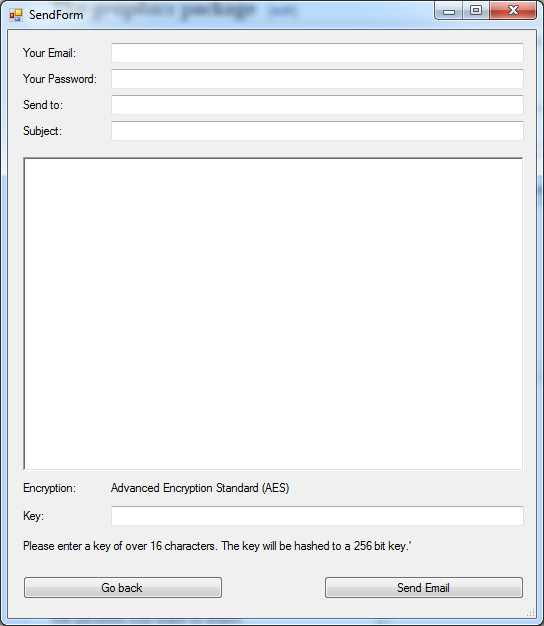
\includegraphics[scale=0.6]{2}
	\caption{Sending an email}
\end{figure}

The main menu of the application allows the user to choose between sending or decrypting an email. Once the user has chosen, the application switches to the appropriate interface. Figure 1.1 is an example of the user interface for sending an email.

\vspace{2.5mm}

After the user enters the information, a variety of steps are taken. First, the key that they have provided is hashed and salted using the SHA-256 algorithm. Afterwards, we format the email in order to let the other user know that they are receiving an encrypted email. Finally, we use implicit TLS in order to have a secure network connection.

\vspace{2.5mm}

We used implicit TLS as the primary cryptographic protocol in sending the email because we wanted full encryption for the connection from the start of the session. In implicit TLS, the following approach is used:
\begin{enumerate}
	\item Client connects to a different port. For example, non encrypted SMTP client connects to port 25 but for implicit TLS, client connects to port 465.
	\item The client establishes an encrypted TLS session immediately upon connecting to the server before exchanging any SMTP data, including reading the server's initial greeting. 
	\item The username and password are sent encrypted.
	\item The session remains encrypted throughout the entire connection.
\end{enumerate}

However, since encryption always consumes more bandwidth and computational resources, there may be instances when you'll want to encrypt only one channel. In that case, you can use explicit SSL which allows you to choose which channel to encrypt.  You can even choose to revert back to a regular (unencrypted) connection and not encrypt any channel at all.

\vspace{2.5mm}

Using TLS/SSL provides us with strong authentication, message privacy, and integrity. TLS/SSL can help to secure transmitted data using encryption. TLS/SSL also authenticates servers and clients to prove the identities of parties engaged in secure communication. It also provides data integrity through an integrity check value. In addition to protecting against data disclosure, the TLS/SSL security protocol can be used to help protect against masquerade attacks, man-in-the-middle attacks, and replay attacks.

\noindent
\section{Cryptographic attacks and their defenses}\label{approach}

\noindent
{\large\textbf{Data Eavesdropping}}

\vspace{1mm}
\noindent
\textit{How it works: }

The majority of network communications occur in an unsecured or plaintext format. This means that an attacker who has gained access to data paths in your network can listen in and interpret the network traffic. In short, eavesdropping is the act of intercepting communications between two points. A specialized program can be used to sniff and record packets of data communications from a network and then subsequently listened to or read using cryptographic tools for analysis and decryption. As an example, Voice over IP (VoIP) calls made using IP-based communication can be picked up and recorded using protocol analyzers and then converted to audio files using other specialized software.

\vspace{2.5mm}
\noindent
\textit{Our defense: }

Our email application uses Transport Layer Security (TLS), and since TLS encrypts the transmission, no data can be eavesdropped. However, TLS cannot prevent eavesdropping if the certificate authority (CA) is not safe, which is not our concern since we are properly checking for valid signed certificates from trusted CAs. However, TLS will not protect against attacks against the endpoints itself. That is, it will not help you if there are bugs in the used TLS stacks, buffer overflows or bugs in the application logic (aka cross-site-scripting). If the attacker manages to compromise the endpoint in some ways (which is unlikely since they have to compromise gmail) he will be able to inject itself into the application to get access to the unencrypted data or to the encryption keys.

\vspace{2.5mm}
\noindent
{\large\textbf{Data Modification}}

\vspace{1mm}
\noindent
\textit{How it works: }

After an attacker has read your data, the next logical step is to alter it. A data modification attack occurs when an attacker modifies the data in the packet without the knowledge of the sender or receiver. Even if you do not require confidentiality for all communications, you do not want any of your messages to be modified in transit. For example, if you go shopping online, you do not want the items, amounts, or billing information to be modified.

\vspace{2.5mm}
\noindent
\textit{Our defense: }

Since our transmission is encrypted, the attacker cannot read our data. This means that the attacker cannot modify it and we are safe from this attack.

\vspace{2.5mm}
\noindent
{\large\textbf{Data Replay}}

\vspace{1mm}
\noindent
\textit{How it works: }

A data replay attack is a form of network attack in which a valid data transmission is maliciously or fraudulently repeated or delayed. Suppose Alice wants to prove her identity to Bob. Bob requests her password as proof of identity, which Alice dutifully provides. Meanwhile, Eve is eavesdropping on the conversation and keeps the password. After the interchange is over, Eve (posing as Alice) connects to Bob; when asked for a proof of identity, Eve sends Alice's password (or hash) read from the last session, which Bob accepts thus granting access to Eve.

\vspace{2.5mm}
\noindent
\textit{Our defense: }

The SSL/TLS channel itself is protected against replay attacks using the MAC. The TLS 1.1 specification Appendix F.2 states: "`To prevent message replay or modification attacks, the MAC is computed from the MAC secret, the sequence number, the message length, the message contents, and two fixed character strings."' Also, TLS requires the client and server to exchange a nonce in the hello message. The implementation should verify that the nonce is never repeated in order to prevent the replay attacks.

\vspace{2.5mm}
\noindent
{\large\textbf{Masquerade Attacks/Identity Spoofing}}

\vspace{1mm}
\noindent
\textit{How it works: }

Most networks and operating systems use the IP address of a computer to identify a valid entity. In certain cases, it is possible for an IP address to be falsely assumed— identity spoofing. The attacker then masquerades as another by falsifying data and gaining an illegitimate advantage. An attacker might also use special programs to construct IP packets that appear to originate from valid addresses. After gaining access to the network with a valid IP address, the attacker can modify, reroute, or delete your data.

\vspace{2.5mm}
\noindent
\textit{Our defense: }

This type of attack is not much of a problem for TLS connections, as TLS authenticates all parties and encrypts all traffic. Using TLS prevents an attacker from performing IP address spoofing on a specific connection (for example, mutual TLS connections). However, an attacker could still spoof the address of the DNS server.

\vspace{2.5mm}
\noindent
{\large\textbf{Man-in-the-Middle Attack}}

\vspace{1mm}
\noindent
\textit{How it works: }

In this attack, an attacker places himself in between a visitor and a web site, impersonating both. With this attack, the browser thinks it is talking to the server on an encrypted channel, and the server thinks it is talking to the browser, but they are both talking to the attacker who is sitting in the middle. All traffic passes through this man-in-the-middle, who is able to read and modify any of the data.

\vspace{2.5mm}
\noindent
\textit{Our defense: }

The certificate authority system is designed to stop the man-in-the-middle attacks. In TLS, the server uses the private key associated with their certificate to establish a valid connection. The server keeps the key secret, so the man-in-the-middle can’t use the site’s real certificate; they have to use one of their own. The attacker has to either convince a certificate authority to sign their certificate, or just use it, as is. A man-in-the-middle trying to use a certificate that is not validated by a known trusted CA should be caught immediately.


\vspace{2.5mm}
\noindent
{\large\textbf{Compromised-Key Attack}}

\vspace{1mm}
\noindent
\textit{How it works: }

A compromised-key attack occurs when the attacker determines the key, which is a secret code or number used to encrypt, decrypt, or validate secret information. This key corresponds to the certificate associated with the server. When the attacker is successful in determining the key, the attacker uses the key to decrypt encrypted data without the knowledge of the sender of the data. 

\vspace{2.5mm}
\noindent
\textit{Our defense: }

If the key is compromised, the attacker still needs access to the actual message in order to decrypt it. Since the message is encrypted twice, once by AES and then by SSL, the message is reasonably secure against this type of attack as the attacker needs two keys.


%%%%%%%%%%%%%%%%%%%%%%%%%%%%%%%%%%%%%%%%%%%%%%%%%%%%%%%%%%%%%
%% BIBLIOGRAPHY AND OTHER LISTS
%%%%%%%%%%%%%%%%%%%%%%%%%%%%%%%%%%%%%%%%%%%%%%%%%%%%%%%%%%%%%
%% A small distance to the other stuff in the table of contents (toc)
\addtocontents{toc}{\protect\vspace*{\baselineskip}}

%% The Bibliography

\clearpage
\addcontentsline{toc}{chapter}{References}
\begin{thebibliography}{9}
\bibitem{networkatks} 
"Common Types of Network Attacks."
\textit{Common Types of Network Attacks. }
Microsoft, n.d. Web. 03 May 2015.
 
\bibitem{northwood} 
Northwood, Chris.
"Cryptography, Attacks and Countermeasures."
\textit{Cryptography, Attacks and Countermeasures}
N.p., n.d. Web. 03 May 2015.

\bibitem{wikitransport}
"Transport Layer Security."
\textit{Wikipedia.} 
 Wikimedia Foundation, n.d. Web. 03 May 2015.

\bibitem{microsoftTLS}
"What Is TLS/SSL?"
\textit{Logon and Authentication.} 
Microsoft, n.d. Web. 03 May 2015.
\end{thebibliography}

%%%%%%%%%%%%%%%%%%%%%%%%%%%%%%%%%%%%%%%%%%%%%%%%%%%%%%%%%%%%%
%% APPENDICES
%%%%%%%%%%%%%%%%%%%%%%%%%%%%%%%%%%%%%%%%%%%%%%%%%%%%%%%%%%%%%
\appendix
%% ==> Write your text here or include other files.
%\input{FileName} %You need a file 'FileName.tex' for this.

\end{document}

